% Chapter: RL for Macroeconomics
% v3 (2026-05-15): unified preliminaries + parallel-structure across all
% paper subsections + difficulty-ordered Option B sequence.
% §1 fixes notation and defines MDP / POMDP / Markov game / MFG with
% common noise / equilibrium concepts once. Each subsequent paper
% subsection follows Setup -> MDP mapping -> Algorithm -> Result.
% Sections proceed from single-agent DSGE to rep-agent RBC sim,
% heterogeneous-agent macro, MFG, ABM, and policy design.
% Tone: understated. Early progress, not a settled toolkit.
% Style: natbib, no em dashes, no colons in prose, no \textbf{},
% no \paragraph*{} headers, no bullet points outside numbered lists.

Reinforcement learning is a recent arrival in macroeconomics. Most of
the algorithms surveyed in this chapter were published in the past
few years, and the literature is small enough that few results have
been independently replicated. The arrival is nevertheless of some
interest, because RL admits two distinct interpretations in a macro
context. As
a solver, RL is a computational tool that finds rational-expectations
or Nash equilibria for models whose state space breaks dynamic
programming. As a behavioural model, RL describes a boundedly-rational
agent who learns a policy from realised utility under no a priori
knowledge of the economy. The two interpretations share the same
training code; the distinction is in what the analyst uses the output
to claim.

This chapter builds up from the simplest case to the hardest, holding
one notation throughout. Section~\ref{sec:macro:setup} fixes the
setup, defines the four problem classes the chapter uses, and lists
the equilibrium concepts. The substantive sections that follow each
cover one or two anchor papers in increasing order of model complexity.
Section~\ref{sec:macro:cjk} treats a single-agent monetary DSGE.
Section~\ref{sec:macro:simulation} reports a textbook
representative-agent RBC simulation that anchors the baseline claim
that RL can match dynamic programming on solvable models.
Section~\ref{sec:macro:solver} scales up to heterogeneous-agent macro
models, where the cross-sectional distribution enters the state.
Section~\ref{sec:macro:mfg} takes the continuum limit to mean field
games with common noise. Section~\ref{sec:macro:abm} covers the
agent-based alternative, in which RL learners are embedded inside
models that keep individual identity rather than taking a mean-field
limit. Section~\ref{sec:macro:policy} closes with applications in
which RL designs macroeconomic policy.
Section~\ref{sec:macro:discussion} reviews open frontiers.

\subsection{Setup and notation}
\label{sec:macro:setup}

We collect the definitions here so that subsequent sections can map a
paper's notation to a single chapter-wide convention without
restating the machinery.

\subsubsection{The agent's MDP}

A Markov decision process (MDP) is a tuple $(\mathcal S, \mathcal A,
P, r, \beta)$ with state space $\mathcal S$, action space
$\mathcal A$, transition kernel $P(s' \mid s, a)$, reward function
$r(s, a) \in \mathbb R$, and discount factor $\beta \in (0, 1)$. A
policy $\pi(a \mid s)$ maps states to action distributions. The
return is $G_t = \sum_{k \ge 0} \beta^k r_{t+k}$, the value is
$V^\pi(s) = \mathbb E^\pi[G_t \mid s_t = s]$, and the Q-function is
$Q^\pi(s, a) = \mathbb E^\pi[G_t \mid s_t = s, a_t = a]$. The optimal
value satisfies the Bellman equation
$V^\star(s) = \max_a \{ r(s, a) + \beta\, \mathbb E[V^\star(s') \mid s,
a]\}$. Reinforcement learning finds an approximately optimal policy
from interaction with the environment rather than from a fully
specified model. We refer to RL algorithms (value iteration,
Q-learning, policy gradient, actor-critic, soft actor-critic, proximal
policy optimisation, deep deterministic policy gradient) by name
without re-deriving them; the algorithmic taxonomy is covered in
Sections~\ref{section:rl_algorithms} and~\ref{section:rl_theory} of
the survey.

\subsubsection{Generalisations used in this chapter}

Four generalisations of the MDP appear in the macro literature
surveyed below.

A partially observed MDP (POMDP) supplements the MDP with an
observation space $\mathcal O$ and an emission distribution
$U(o \mid s)$. The agent does not see the state $s$ directly; it
conditions its policy on the observation history $o_{0:t}$, typically
through a recurrent network or a sufficient statistic. POMDPs arise
in macro whenever a household sees only prices or summary statistics
rather than the full cross-sectional distribution.

A Markov game extends the MDP to $n$ agents who share the state but
choose actions independently. Each agent $i \in \{1, \ldots, n\}$ has
its own action space $\mathcal A_i$ and reward $r_i(s, a)$, where
$a = (a_1, \ldots, a_n)$ is the joint action. Each agent treats the
other agents' policies as part of a non-stationary environment and
maximises its own return. Two-level games (a planner and a population
of agents) are a special case.

A mean field game with common noise takes the continuum limit
$n \to \infty$. A representative agent interacts with the
cross-sectional distribution $\mu \in \Delta(\mathcal S)$ of
individual states and with a common noise $z \in \mathcal Z$ that
captures aggregate shocks. The individual transition is
$T(s' \mid s, a, \mu, z)$; the mean field evolves under
$\mu_{t+1} = \Phi^\pi(\mu_t, z_t)$ for an operator $\Phi^\pi$ induced
by the policy. The continuum limit makes the otherwise exponential
per-agent state space tractable at the cost of losing finite-population
effects.

A multi-objective MDP replaces the scalar reward $r$ with a vector
$r \in \mathbb R^d$. The solution concept is a Pareto front rather
than a single optimum.

\subsubsection{Equilibrium concepts}

A policy $\pi^\star_i$ is a best response to the other agents'
policies $\pi_{-i}$ when $V_i^{(\pi^\star_i, \pi_{-i})}(s) \ge
V_i^{(\pi'_i, \pi_{-i})}(s)$ for every alternative $\pi'_i$. A Nash
equilibrium is a profile $(\pi^\star_1, \ldots, \pi^\star_n)$ in which
every component is a best response to the others. A mean-field Nash
equilibrium is the continuum analogue, in which the representative
agent's policy is a best response to the cross-sectional distribution
it induces. A restricted perceptions equilibrium is a best response
within a restricted policy class, for example policies that condition
on prices but not on the full distribution; it is weaker than
rational expectations and is the natural equilibrium concept for the
SRL approach in Section~\ref{sec:macro:solver}. An
$\varepsilon$-equilibrium weakens Nash by an $\varepsilon$ slack on
each player's incentive. Exploitability, $\sup_{\pi'} V^{\pi'} -
V^\pi$ evaluated at the current mean field, is the natural
convergence metric in MFG-RL because it upper-bounds the gap to a
mean-field Nash equilibrium.

\subsubsection{Notation summary and reading guide}

Throughout the chapter we use $s$ for state, $a$ for action, $r$ for
reward, $\pi$ for policy, $V$ and $Q$ for values, $\beta$ for the
discount factor, $P$ or $T$ for the transition kernel,
$\mu \in \Delta(\mathcal S)$ for the cross-sectional distribution,
$z \in \mathcal Z$ for the aggregate shock or common noise, $p$ for
the equilibrium price vector when explicit, $\theta$ for policy
parameters, $\phi$ for auxiliary parameters when a second network is
needed (a critic in single-agent RL, a planner in two-level RL), $n$
for the number of agents in a Markov game, and $i$ for an agent
index. Algorithm-specific scalars (training-step counts $N$, $T$,
trajectory counts $E$) are introduced inside the relevant algorithm
boxes.

The chapter applies RL to macro models under two interpretations,
introduced above and used without further comment hereafter. Under
the solver interpretation, the policy network is a numerical device
for finding an equilibrium that closed-form or DP-based methods
cannot reach. Under the behavioural interpretation, the policy
network is the household's actual cognition, learning a policy from
realised utility under no prior model knowledge.
Sections~\ref{sec:macro:cjk} and~\ref{sec:macro:abm} lean on the
behavioural interpretation; Sections~\ref{sec:macro:solver}
and~\ref{sec:macro:mfg} lean on the solver interpretation;
Section~\ref{sec:macro:policy} uses one or the other depending on
whether the planner is the focus.

A growing parallel literature uses deep learning rather than
reinforcement learning to solve heterogeneous-agent and DSGE models
by training networks to satisfy equilibrium equations as nonlinear
regression objectives \citep{Maliar2021dl, Azinovic2022den,
Azinovic2026sequence, Kase2025hank, Kase2025gem,
HallHoffarth2023constraints, Carmona2021mfg, Fang2026dpi,
Thoeni2026nmfg}; \citet{Fernandez2024dl} survey this line. The
distinction is that those methods compute equation residuals offline,
while RL trains the network from a reward signal under the agent's
own policy. The chapter restricts attention to the RL lens and
surfaces the equation-residual literature only as a comparison point
where relevant.

\subsection{Deep RL in a monetary DSGE}
\label{sec:macro:cjk}

\citet{Chen2021drl} apply deep RL to the \citet{Benhabib2001} model of
monetary-fiscal interaction. A representative household solves
\begin{equation}
\max\, \mathbb{E}_0 \sum_{t=0}^{\infty} \beta^t \bigl[\,u(c_t) + v(m_t) - w(n_t)\,\bigr]
\quad \text{s.t.} \quad c_t + m_t + b_t = w_t n_t - \tau_t + \frac{R_{t-1} b_{t-1} + m_{t-1}}{\pi_t},
\label{eq:macro:cjk-household}
\end{equation}
where $m_t = M_t/P_t$ is real money, $b_t = B_t/P_t$ is real bonds,
$\tau_t$ is a lump-sum tax, $w_t$ is the real wage, $\pi_t =
P_t/P_{t-1}$ is gross inflation, and output is linear in labour,
$y_t = \varepsilon^y_t n_t$, with $\varepsilon^y_t$ an i.i.d.\
technology shock. Fiscal policy follows a Leeper-style rule
$\tau_t = \gamma_0 + \gamma\, b_{t-1} + \varepsilon^\tau_t$ and
monetary policy follows a global nonlinear interest-rate rule
$R_t = f(\pi_t)\, \varepsilon^R_t$ with $f$ strictly positive and
strictly increasing. The deterministic Fisher equation $R = \pi/\beta$
intersects $f(\pi)$ at the inflation target $\pi^\star$ and at a
liquidity trap $\pi_L$.\footnote{Each policy rule is locally active
or passive depending on the sign of a coefficient. Fiscal policy is
active when $\gamma < \beta^{-1} - 1$. Monetary policy is locally
active at inflation $\pi$ when $f'(\pi) > \beta^{-1}$. The
cross-product of the two stances generates four regimes, of which the
doubly-passive case is locally indeterminate under rational
expectations and the doubly-active case is locally explosive.
\citet{EvansHonkapohja2005} show that recursive-least-squares
adaptive learning reaches only the determinate regimes.}

In the chapter's MDP notation, the household's state is
$s_t = (m_{t-1}, b_{t-1}, \pi_{t-1}, c_{t-1}, n_{t-1},
\varepsilon^\tau_t, \varepsilon^R_t, \varepsilon^y_t)$, the action
$a_t = (c_t, b_t, n_t)$ is a continuous tuple of consumption, bond
holdings, and labour, the reward $r_t = u(c_t) + v(m_t) - w(n_t)$ is
the instantaneous utility, and the transition $P(s_{t+1} \mid s_t,
a_t)$ is induced by the household's intertemporal Euler equation
\begin{equation}
u'(c_t) \;=\; \beta\, R_t\, \mathbb{E}_t\!\left[\frac{u'(c_{t+1})}{\pi_{t+1}}\right]
\label{eq:macro:cjk-euler}
\end{equation}
together with the equilibrium fiscal-monetary rules and the exogenous
shock processes. The policy is learned by soft actor-critic
\citep{Haarnoja2018}.\footnote{SAC is an off-policy maximum-entropy
actor-critic. The Gaussian actor $\pi_\theta$ and the Q-function
$Q_\phi$ are deep neural networks trained by stochastic gradient
descent on minibatches drawn from a replay buffer. The critic update
follows the temporal-difference loss with a target network and the
actor update is the reparameterised maximum-entropy gradient.}

Algorithm~\ref{alg:macro:cjk-sac} gives the training loop. The
schedule consists of an initial burn-in phase with uniformly sampled
actions, followed by entropy-regularised on-policy exploration.
Episodes are reset by sampling an initial state from a region of
interest and terminate either at the per-episode cap or when the
running utility improvement falls below a tolerance.\footnote{The
paper does not publish a single hyperparameter table; the burn-in
length, total training step count, batch size, and learning rate are
reported across appendix tables indexed by experiment.}

\begin{algorithm}[t]
\caption{Soft Actor-Critic for the monetary DSGE household, after \citet{Chen2021drl}}
\label{alg:macro:cjk-sac}
\begin{algorithmic}[1]
\Require burn-in $N_{\text{burn}}$; total training steps $N_{\text{train}}$; per-episode cap $N^{\max}_{\text{epi}}$; utility tolerance $d^{\min}_u$; test interval $N_{\text{interval}}$
\State Initialise actor $\theta$, critic $\phi$, and step counter $\tau \leftarrow 0$
\While{$\tau < N_{\text{train}}$}
  \State Begin a new training episode with $s_\tau$ drawn uniformly from a region of interest
  \For{up to $N^{\max}_{\text{epi}}$ steps within the episode}
    \State Sample $a_\tau$ uniformly at random if $\tau < N_{\text{burn}}$; otherwise $a_\tau \sim \pi_\theta(\cdot \mid s_\tau)$ from the entropy-regularised policy
    \State Step the economy via household FOCs and equilibrium fiscal-monetary rules; store $(s_\tau, a_\tau, r_\tau, s_{\tau+1})$ in the replay buffer
    \State Update $\phi$ on a minibatch via temporal-difference loss; update $\theta$ via reparameterised maximum-entropy gradient
    \State $\tau \leftarrow \tau + 1$; terminate the episode if the utility improvement falls below $d^{\min}_u$
    \If{$\tau \bmod N_{\text{interval}} = 0$}
      \State Snapshot $(\theta, \phi)$ and run deterministic test episodes
    \EndIf
  \EndFor
\EndWhile
\State \Return trained $(\theta, \phi)$
\end{algorithmic}
\end{algorithm}

\citet{Chen2021drl} report that the DRL household reaches a stationary
policy in all four monetary-fiscal regimes. Under active-monetary and
passive-fiscal policy, the DRL policy converges to $\pi^\star$. Under
passive-monetary and active-fiscal policy, it converges to $\pi_L$.
In the doubly-passive regime (locally indeterminate under rational
expectations) and the doubly-active regime (locally explosive), the
DRL policy still settles into a stationary equilibrium. The
interpretation offered is that the deep policy is constrained by the
agent's global utility-maximisation problem rather than by the
linearised dynamics around a particular steady state. The result is
robust to small monetary, fiscal, and labour-supply shocks. The
finding is a within-paper claim on a single calibration, and an
independent replication on the same Benhabib environment has not
been published. Under the behavioural interpretation of
Section~\ref{sec:macro:setup}, the result is that boundedly-rational
deep-RL households can sustain stationary outcomes in regimes that
recursive-least-squares adaptive learning cannot.

\subsection{Simulation: representative-agent RBC under DP and DRL}
\label{sec:macro:simulation}

Before scaling to harder models, we check that RL matches dynamic
programming on a problem for which DP is the right tool. The
environment is a standard representative-agent stochastic RBC. The
household chooses consumption $C_t$ and saves the residual, with
capital evolving as $K_{t+1} = (1-\delta) K_t + A_t K_t^\alpha - C_t$
and total factor productivity following $\log A_{t+1} = \rho \log A_t
+ \varepsilon_{t+1}$ for $\varepsilon_{t+1} \sim \mathcal{N}(0,
\sigma^2)$. Utility is $u(C_t) = \log C_t$. Parameters are calibrated
as $\beta = 0.96$, $\alpha = 0.36$, $\delta = 0.10$, $\rho = 0.95$,
$\sigma = 0.007$, with horizon $T = 200$. The deterministic steady
state is $K^\star = 4.29$, $C^\star = 1.26$.

In the chapter's MDP notation the state is $s = (K, A)$, the action
is $a = C$, the reward is $r = \log C$, and the transition is the
capital accumulation equation together with the AR(1) for TFP. Four
methods are compared: a Blanchard-Kahn log-linearisation around the
deterministic steady state (KPR), value-function iteration on a
$400 \times 41$ tensor grid with a Tauchen-discretised TFP process
(VFI), proximal policy optimisation with a Gaussian actor (PPO), and
deep deterministic policy gradient (DDPG).\footnote{Both RL methods
use a 64-64 multilayer perceptron for actor and critic. Each is
trained from scratch with $10$ independent seeds. Every method is
evaluated on a fixed set of $30$ initial conditions $(K_0, A_0) \sim
\mathcal{U}[0.5, 8] \times \mathcal{U}[0.95, 1.05]$ and shock paths
$\{\varepsilon_t\}_{t=1}^T$, identical across methods, so cross-method
differences are not driven by evaluation noise. The training budgets
and convergence-monitoring schedules are recorded in the simulation
script.}

Table~\ref{tab:macro:rbc-results} reports mean episode return,
standard error, and policy mean-squared error against VFI. KPR
matches VFI to within $0.001$ in policy MSE and within statistical
noise on mean return. PPO converges to within the standard error of
VFI with a policy MSE of $0.009$. DDPG attains a mean return within
$2\%$ of VFI but with roughly double the cross-seed standard error
and a policy MSE of $0.037$, consistent with the known sensitivity
of deterministic policy gradient methods to hyperparameter and
initialisation choices. Figure~\ref{fig:macro:rbc-curves} traces the
learning curves of PPO and DDPG against the VFI and KPR horizontal
benchmarks. Both RL methods approach the analytical benchmark within
their respective training budgets. The result is what one would hope
on a model this small. It is not a demonstration that RL replaces
dynamic programming; it is a check that RL does not fail it on the
textbook case.

\begin{table}[ht]
\centering
\begin{tabular}{lrrrr}
\toprule
Method & Mean return & SE & Policy MSE vs VFI & Wall clock \\
\midrule
KPR & 45.88 & 0.587 & 0.0004 & $-$ \\
VFI & 45.86 & 0.589 & 0.0000 & 13.8 s \\
PPO & 45.82 & 0.843 & 0.0087 & 32.9 s \\
DDPG & 45.17 & 1.476 & 0.0365 & 579.4 s \\
\bottomrule
\end{tabular}

\caption{Representative-agent RBC under four methods. Mean episode return averaged over 30 evaluation episodes with shared initial conditions and shock paths. Standard error across 10 training seeds for PPO and DDPG, across 30 evaluation episodes for KPR and VFI. Policy mean-squared error reported against VFI consumption on 1000 random states drawn uniformly from the evaluation support.}
\label{tab:macro:rbc-results}
\end{table}

\begin{figure}[ht]
\centering
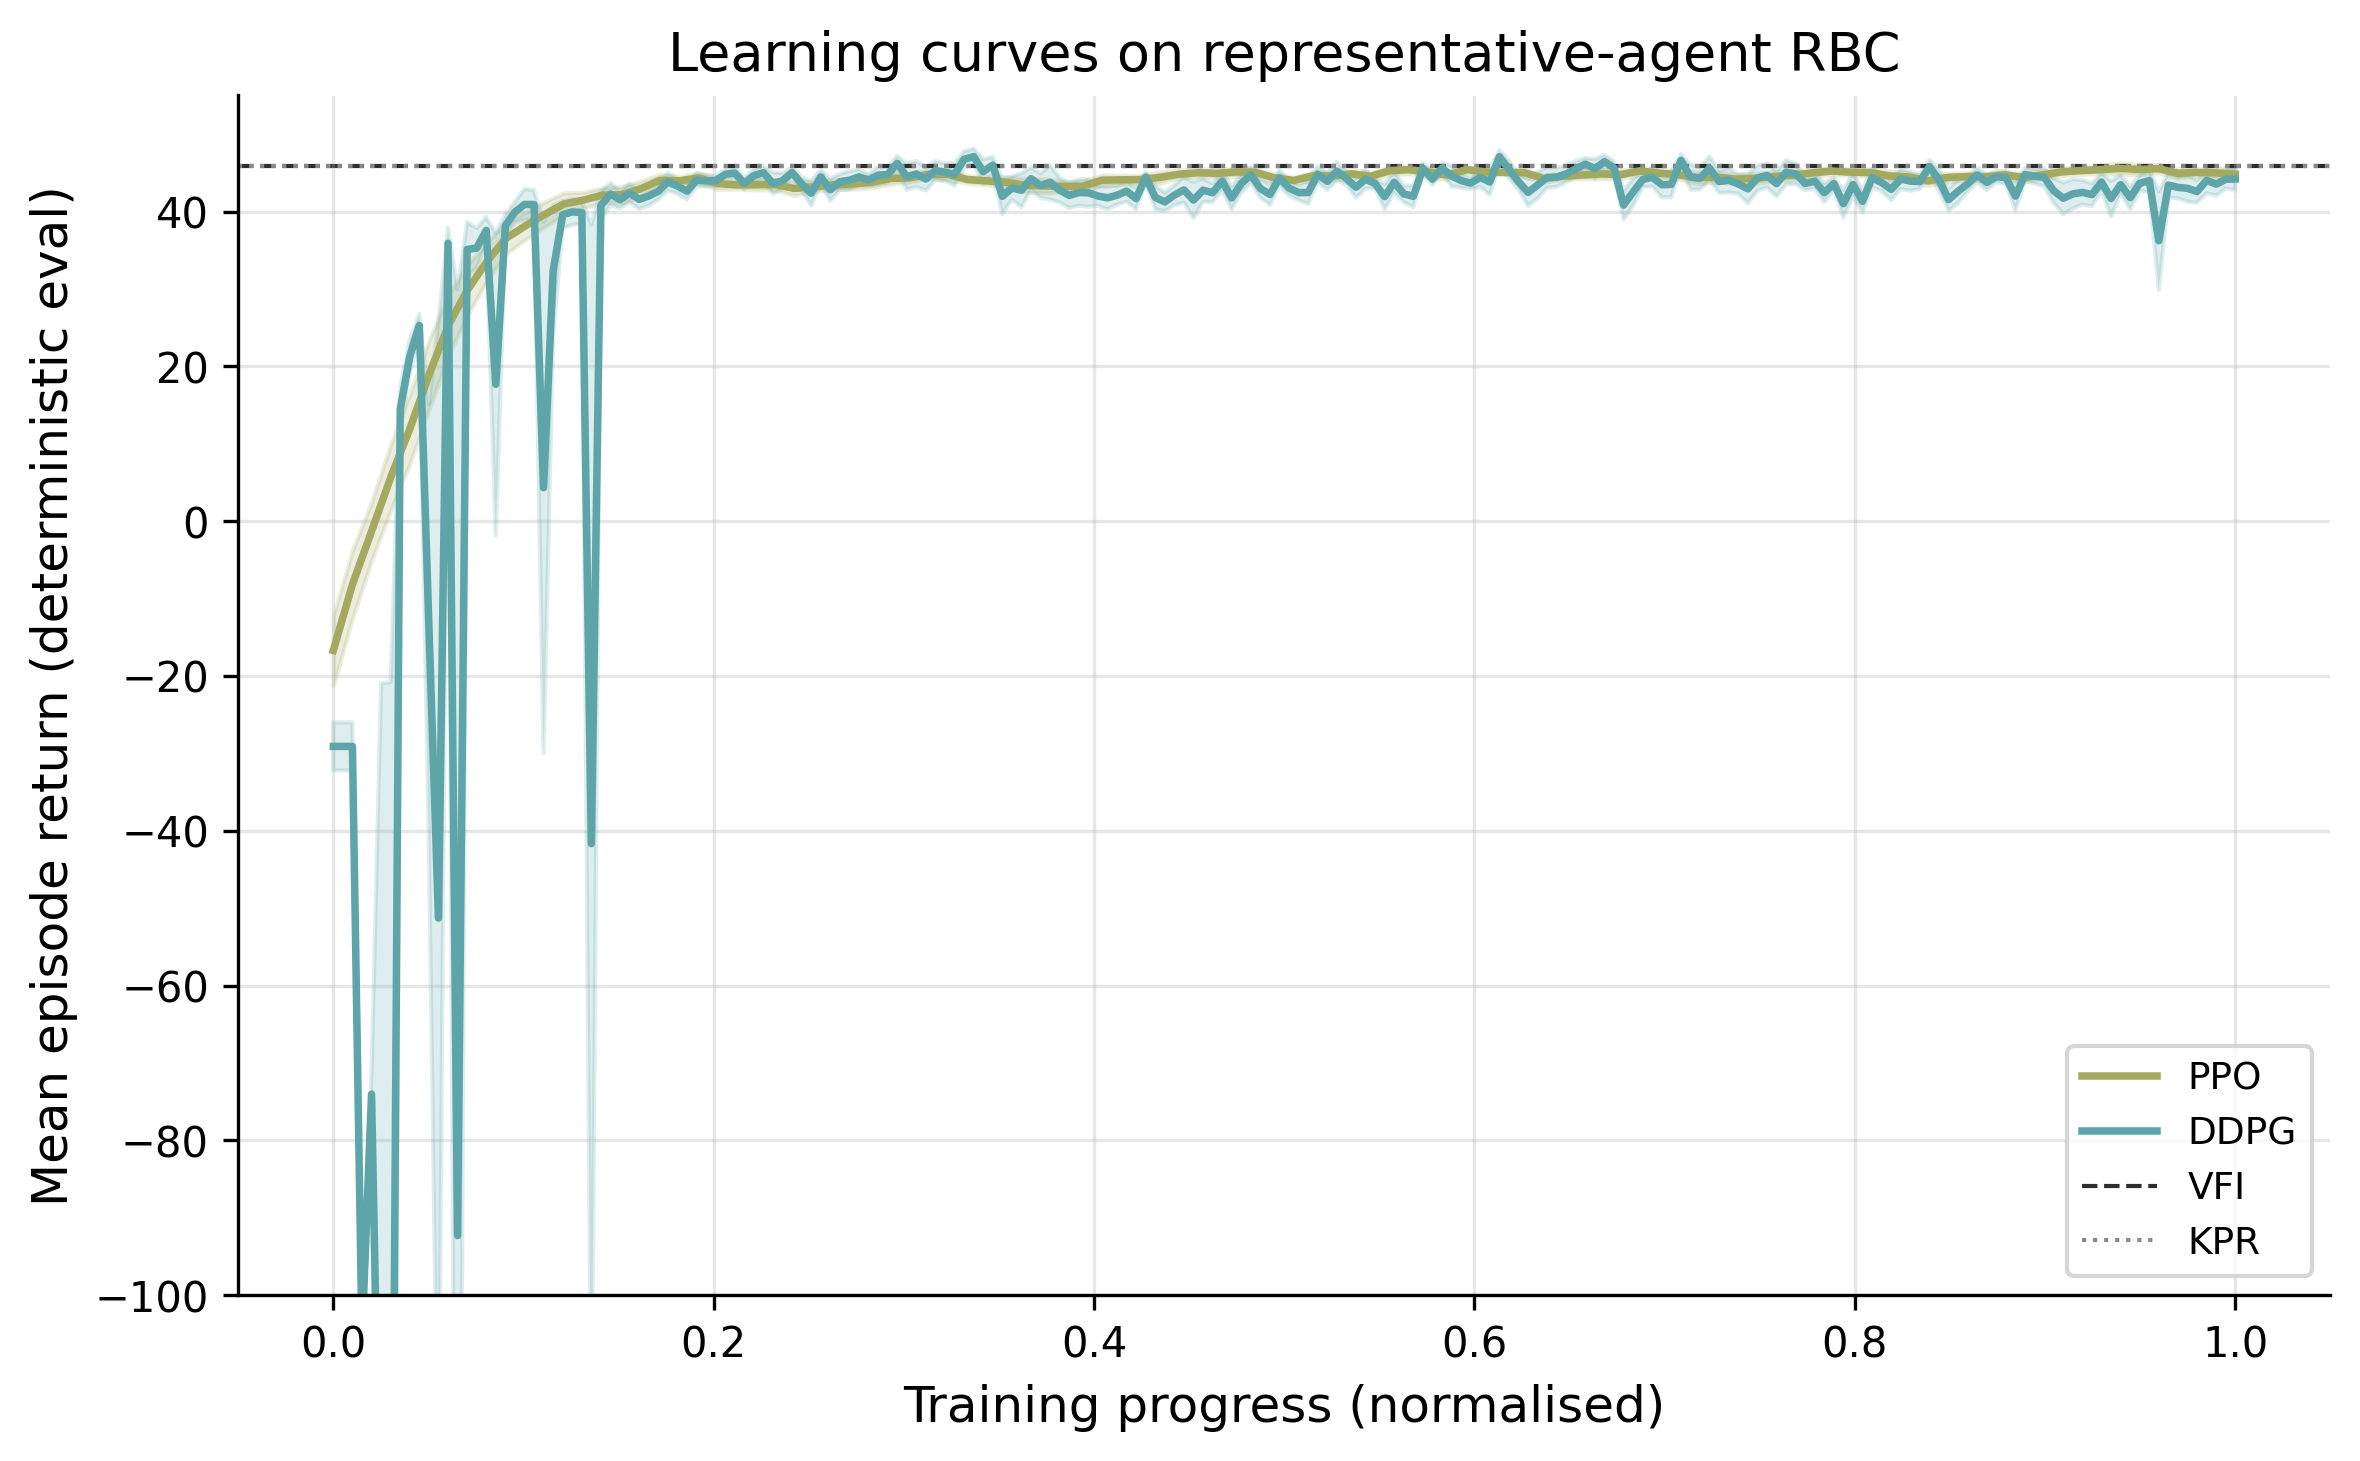
\includegraphics[width=0.85\linewidth]{../ch06_macro/sims/rbc_dp_vs_drl_learning_curves.png}
\caption{Mean deterministic-evaluation return as a function of normalised training progress for PPO (olive) and DDPG (cyan), shaded by cross-seed standard error across ten training seeds. Horizontal lines mark the VFI benchmark mean return (dashed black) and the KPR log-linear benchmark (dotted gray).}
\label{fig:macro:rbc-curves}
\end{figure}

\subsection{RL as a global solver for heterogeneous-agent macro models}
\label{sec:macro:solver}

Heterogeneous-agent (HA) macro models replace the representative
agent of Section~\ref{sec:macro:simulation} with a continuum of
households facing uninsurable idiosyncratic shocks on top of an
aggregate shock. Canonical examples are \citet{Aiyagari1994},
\citet{KrusellSmith1998}, and \citet{KaplanMollViolante2018}. The
state of the agent's problem now includes the cross-sectional
distribution $\mu_t \in \Delta(\mathcal S)$ of individual states,
because equilibrium prices depend on $\mu_t$ and the distribution
itself depends on the policy. Dynamic programming runs on an
infinite-dimensional state and the value function lives on
$\mathcal S \times \Delta(\mathcal S) \times \mathcal Z$. The
traditional macro response summarises $\mu_t$ by a handful of moments
\citep{KrusellSmith1998} or linearises around a stationary
equilibrium \citep{Reiter2009, Auclert2021}. Both reductions impose
ex ante which features of the distribution matter.

\citet{Yang2025srl} propose Structural Reinforcement Learning (SRL),
which sidesteps the distribution entirely. The structural assumption
is that the household knows its own budget constraint, preferences,
and idiosyncratic shock process exactly. The only unknown part of
the environment from the household's point of view is the joint
process for equilibrium prices and aggregate shocks. SRL trains the
policy by simulating the full economy and treating prices as
exogenous to the agent through a stop-gradient. The Wold
representation theorem justifies dropping $\mu$ from the agent's
state in favour of the price history; under rational expectations
the price history is a sufficient statistic for whatever a
forward-looking household needs from $\mu$. \citet{Han2022deepham},
the immediate predecessor of SRL, kept the full cross-sectional
distribution $\mu$ in the agent state via a deep-network policy that
conditions on $\mu$ directly; SRL replaces $\mu$ with prices.

In the chapter's MDP notation the SRL household's state is
$s_t = (b_t, y_t, z_t, p_t)$, with $b_t$ wealth, $y_t$ the
idiosyncratic productivity shock, $z_t$ the aggregate shock, and
$p_t$ the equilibrium price vector. The action is $a_t = c_t$,
consumption, with savings $b_{t+1}$ determined residually by the
budget. The next state is generated by three structural pieces: the
budget constraint for $b_{t+1}$, the exogenous Markov chain for
$(y_{t+1}, z_{t+1})$, and the market-clearing update $p_{t+1} =
P^\star(\mu_{t+1}, z_{t+1})$ that the agent treats as exogenous. The
reward is $r_t = u(c_t)$. The policy class is restricted to
$\pi(s, z, p)$, which means the agent never conditions on $\mu$ at
any step. \citet{Yang2025srl} call the resulting fixed point a
sequential restricted perceptions equilibrium: given the price
process induced by $P^\star$, the policy $\pi^\star$ maximises
expected discounted utility within the restricted class, and market
clearing holds at $p_t = P^\star(\mu_t, z_t)$ for every $t$. Agents'
price beliefs are statistically consistent with realised prices on
the equilibrium path, and the equilibrium is a fixed point in policy
space rather than in the perceived-law-of-motion regression of
Krusell-Smith.

Training uses the structural policy gradient (SPG) algorithm of
Algorithm~\ref{alg:macro:spg}.\footnote{The cross-sectional
distribution rolls forward to compute prices while a separate
value-computation distribution rolls forward to score the policy.
The policy is parameterised as a tabular vector $\theta \in \mathbb
R^{J \times K \times L}$ on the discretised $(s, z, p)$ grid. The
Monte Carlo value is differentiated analytically by backpropagating
through the known one-step transition matrix $A_\pi(z, p)$, the
discrete instantiation of the chapter-general transition kernel
restricted to the policy and grid. Convergence is monitored by the
$\ell_\infty$ distance between successive policy iterates and is
declared at a tolerance $\varepsilon$.}

\begin{algorithm}[t]
\caption{Structural Policy Gradient (SPG) for HA macro models}
\label{alg:macro:spg}
\begin{algorithmic}[1]
\Require initial tabular policy $\theta_0 \in \mathbb{R}^{J \times K \times L}$ on the $(s, z, p)$ grid; step sizes $\{\eta_k\}$; trajectory count $N$; horizon $T$; initial distributions $\psi_g, \psi_z$; convergence tolerance $\varepsilon$
\For{$k = 0, 1, 2, \ldots$}
  \State Sample $N$ initial conditions $(\mu^n_0, z^n_0) \sim (\psi_g, \psi_z)$ for $n = 1, \ldots, N$
  \State Initialise the value-computation distribution $d^n_0 = d_0$, uniform over the individual-state grid
  \For{$n = 1, \ldots, N$}
    \For{$t = 0, 1, \ldots, T-1$}
      \State Compute the equilibrium price $p^n_t = P^*(\mu^n_t, z^n_t)$ from market clearing, with a stop-gradient applied to $p^n_t$
      \State Roll the cross-sectional distribution: $\mu^n_{t+1} = A_{\pi_\theta}(z^n_t, p^n_t)^\top \mu^n_t$ (used only to update prices)
      \State Roll the value-computation distribution: $d^n_{t+1} = A_{\pi_\theta}(z^n_t, p^n_t)^\top d^n_t$ (used only for the value)
      \State Sample the next aggregate shock $z^n_{t+1} \sim \Xi(\cdot \mid z^n_t)$
    \EndFor
  \EndFor
  \State Form the Monte Carlo value $\widehat{v}^{\pi}(\theta_k) = \dfrac{1}{N}\sum_{n=1}^N \sum_{t=0}^{T-1} \beta^t \,\bigl\langle d^n_t,\, u^{\pi_\theta}(z^n_t, p^n_t)\bigr\rangle$
  \State Compute the analytic gradient $\nabla_\theta \widehat{v}^{\pi}(\theta_k)$ by backpropagating through $A_{\pi_\theta}$ with prices held fixed by the stop-gradient
  \State Update $\theta_{k+1} \leftarrow \theta_k + \eta_k \nabla_\theta \widehat{v}^{\pi}(\theta_k)$
  \If{$\|\theta_{k+1} - \theta_k\|_\infty < \varepsilon$}
    \State \Return $\theta_{k+1}$
  \EndIf
\EndFor
\end{algorithmic}
\end{algorithm}

\citet{Yang2025srl} report runtimes on a single A100 GPU. Krusell-Smith
converges in roughly $55$ seconds and the authors report that its
dynamics match the deep-learning rational-expectations benchmark.
The Huggett model with aggregate risk, which has a nontrivial
market-clearing condition for bonds, converges in roughly $75$
seconds. A one-account HANK model with a forward-looking Phillips
curve and sticky prices converges in roughly three
minutes. Allowing agents to condition on a short price history rather
than only the current price does not change the solution materially,
which suggests that current prices encode most of the information
relevant for behaviour in these calibrations. The three benchmark
numbers are within-paper and have not been replicated independently
at the time of writing.

\subsection{Mean Field Games as a large-population RL problem}
\label{sec:macro:mfg}

The mean-field game generalisation of Section~\ref{sec:macro:setup}
applies when large populations of identical, anonymous agents
interact through aggregate quantities. Direct multi-agent RL does
not scale, since the joint state and action spaces grow exponentially
in $n$. Taking the continuum limit reduces the problem to a single
representative agent whose environment includes the population
distribution $\mu \in \Delta(\mathcal S)$ and the common noise $z$.
The RL problem is to find a policy that is a best response to the
distribution it induces under the noise process. Convergence to a
mean-field Nash equilibrium is monitored by exploitability.

\subsubsection{Recurrent Structural Policy Gradient}
\label{sec:macro:rspg}

\citet{Wibault2026rspg} propose the Recurrent Structural Policy
Gradient (RSPG) algorithm for partially observable mean field games
with common noise. In macroeconomic applications agents typically
observe equilibrium prices but not the cross-sectional distribution,
so the natural formulation is a POMFG. RSPG exploits the fact that
individual transitions $T(s' \mid s, a, \mu, z)$ are known to the
agent (the household knows its own budget constraint and
idiosyncratic shock process), while the aggregate process for
$(\mu, z)$ must be learned. The setting therefore sits between
dynamic programming, which would integrate over both, and model-free
RL, which would sample both.

In chapter notation the POMFG with common noise is a tuple
$(p_{\mu_0}, p_{z_0}, \mathcal S, \mathcal Z, \mathcal A, T, \Xi, R,
\beta, U, \mathcal O)$, combining the MFG primitives of
Section~\ref{sec:macro:setup} with the POMDP observation pair
$(U, \mathcal O)$ and a common-noise transition $\Xi(\cdot \mid z)$.
The mean field evolves under the analytic operator
$\mu_{t+1} = \Phi^\pi(\mu_t, z_t)$ with $(s, s')$ entry
$\mathbb{E}_{a \sim \pi}[T(s' \mid s, a, \mu, z)]$. The RSPG
architectural choice is to restrict the policy memory to a history
of shared aggregate observations $o_{0:t}$, parameterised as the
hidden state of a recurrent neural network. The reduced policy
$\pi(a \mid s, h(o_{0:t}))$ retains history-dependence while keeping
the asymptotic cost of the analytic mean-field update independent of
the individual state.

For an initial common-noise distribution $p_{z_0}$, RSPG samples $E$
trajectories in parallel, rolls out the endogenous mean field
$\mu^\pi_{0:T}$ via the analytic operator $\Phi^\pi$, and computes
the discounted return
\begin{equation}
J^\pi \;=\; \mathbb{E}_{z_{0:T} \sim \Xi}\,\Bigl[\sum_{t=0}^{T-1} \beta^t \, \langle \mu^\pi_t,\; R(\cdot,\, \pi,\, \mu^\pi_t,\, z_t)\rangle\Bigr].
\label{eq:macro:rspg-return}
\end{equation}
Gradients flow through the individual transitions $T$ and the
expected-reward over actions. Gradients do not flow through the
mean-field transitions; the analytic mean-field update is treated as
a fixed environment, mirroring SRL's treatment of equilibrium
prices.\footnote{The training loop is parameterised by the
common-noise-trajectory batch size $E$, the rollout horizon $T$, and
the RNN hidden dimension. Convergence is monitored by exploitability,
the gap between the value of a best-response policy and the value of
the agent's current policy at the current mean field. The
exploitability metric requires a separate best-response oracle that
\citet{Wibault2026rspg} train as a single-agent RL agent against the
frozen mean-field path; reported exploitabilities are therefore upper
bounds.}

\begin{algorithm}[t]
\caption{Recurrent Structural Policy Gradient (RSPG)}
\label{alg:macro:rspg}
\begin{algorithmic}[1]
\Require initial recurrent policy $\theta_0$; trajectories $E$; horizon $T$
\For{$k = 0, 1, 2, \ldots$ until convergence}
  \State Sample $E$ common-noise trajectories $z^e_{0:T}$ with $z^e_0 \sim p_{z_0}$ and $z^e_{t+1} \sim \Xi(\cdot \mid z^e_t)$
  \State Roll forward $\mu^e_{t+1} = \Phi^{\pi_\theta}(\mu^e_t, z^e_t)$ analytically, with policy memory $h^e_{t+1} = \mathrm{RNN}(h^e_t, o^e_t)$
  \State Form the sample return $\widehat{J}(\theta_k)$ from \eqref{eq:macro:rspg-return} averaged over $e = 1, \ldots, E$
  \State Update $\theta_{k+1} \leftarrow \theta_k + \eta_k \nabla_\theta \widehat{J}(\theta_k)$ with gradients flowing through $T$ and $R$ only
\EndFor
\State \Return $\theta^*$
\end{algorithmic}
\end{algorithm}

\citet{Wibault2026rspg} evaluate RSPG on partially observable
Linear-Quadratic, Beach-Bar, and Krusell-Smith environments. Across
the three, RSPG attains the lowest or second-lowest exploitability
among the algorithms compared and converges roughly an order of
magnitude faster in wall-clock time than independent and recurrent
PPO baselines. Finite-horizon agents under RSPG spend wealth just
before episode end, pushing interest rates up and wages down.
Memoryless variants of SPG and IPPO do not show this pattern. The
paper positions RSPG as the first method to solve a partially
observable Krusell-Smith model in which agents observe prices but
not the cross-sectional distribution; the comparison set is small
and the result is within-paper.

\subsubsection{Offline, asynchronous, and non-stationary MFG-RL}
\label{sec:macro:other-mfg-rl}

Three recent algorithms extend MFG-RL along orthogonal axes.
\citet{Brunnbauer2024offmmd} learn an equilibrium policy from a
static dataset of past trajectories without online interaction, by
adapting Munchausen online mirror descent to offline data with an
overestimation-mitigating regulariser; their experiments are on
crowd-exploration and navigation, not macro.
\citet{YangShan2026tmf} drop the synchronous-move assumption by
replacing the mean-action statistic $\bar a$ with the population
distribution $\mu \in \Delta(\mathcal O)$, derive a TMF Bellman
equation, and prove an $O(1/\sqrt{N})$ finite-population
exploitability bound that holds for any batch size of acting agents.
\citet{Magnino2025nonstationary} consider non-stationary
continuous-space MFGs and report roughly an order-of-magnitude
reduction in sampling cost on their benchmarks via a fictitious-play
loop with a time-conditional normalising flow on the equilibrium
density.\footnote{\citet{Peng2025mfcg} apply PPO with generalised
advantage estimation and target networks to mean-field control
games, a hybrid that combines internal coordination as in mean-field
control with external competition as in MFGs.}

\subsection{Agent-based macroeconomic models with RL agents}
\label{sec:macro:abm}

The methods above take the continuum limit and let market clearing
coordinate behaviour through prices. The agent-based paradigm keeps
individual identity, replaces market clearing with explicit
search-and-match protocols, and lets macro dynamics emerge from the
local interactions of bounded-rational agents. The setting is a
Markov game in the sense of Section~\ref{sec:macro:setup}, with $n$
heterogeneous agents whose actions are coordinated by hand-coded
protocols rather than by a central market. RL enters this paradigm
under the behavioural interpretation: it replaces some or all of the
hand-coded behavioural rules with policies trained from realised
payoffs.

\subsubsection{Multi-agent RL on heterogeneous RBC}
\label{sec:macro:marl-rbc}

\citet{Gabriele2026marlbc} build MARL-BC, an $n$-household RBC in
which the representative-agent RBC and the Krusell-Smith mean-field
economy appear as limit cases. Each household chooses a consumption
fraction and labour supply at every period. Production is
Cobb-Douglas in productivity-weighted aggregate capital and labour.
In the chapter's Markov-game notation, the state is shared across
agents and contains aggregate capital, labour, and the per-agent
productivity draws; each agent's action is its consumption fraction
and labour choice; each agent's reward is the log-plus-leisure
utility
\begin{equation}
r^i_t \;=\; \log c^i_t + b\,\log(1 - \ell^i_t).
\label{eq:macro:marl-bc-reward}
\end{equation}
The authors benchmark PPO, SAC, DDPG, and TD3 and report that the
off-policy methods are more sample-efficient than PPO on the
configurations they
test.\footnote{Sample efficiency is reported in terms of environment
steps to reach a fixed return threshold. The exact threshold and the
number of seeds vary across the three population configurations,
$n=1$, $n=20$ ex-ante identical, $n=20$ heterogeneous. The paper
does not provide a single hyperparameter table for the four
algorithms.} With $n = 1$ the framework reproduces the textbook RBC
solution. With a large population of ex-ante identical agents (in
their largest run, on a $23 \times 23$ productivity grid yielding
$n = 529$) it reproduces the Krusell-Smith mean-field wealth
distribution and aggregate dynamics. With a population of
heterogeneous agents it produces wealth and consumption distributions
that mean-field methods cannot represent.

\citet{Curry2022marl} consider a richer micro-founded RBC with $100$
worker-consumers, $10$ firms, and a tax-setting government,
formulated as a partially observable Markov game in which firms set
prices and wages and goods are rationed proportionally if demand
exceeds supply. Each agent type is trained by independent PPO with
parameter sharing within type, accelerated by the WarpDrive GPU
framework.\footnote{Without a curriculum, independent learners fail
to recover non-trivial behaviour. A multi-phase curriculum that
stages consumer, firm, and government training recovers non-trivial
$\varepsilon$-meta-equilibria. The $\varepsilon$ metric is evaluated
by training single-agent best-response oracles against frozen others,
so reported values are upper bounds.} In the open-economy variant
with an external export market, the model exhibits multiple
qualitatively distinct $\varepsilon$-meta-equilibria.

\subsubsection{RL agents inside macro ABMs}
\label{sec:macro:rmabm}

\citet{Brusatin2024rmabm} extend an existing macroeconomic ABM with
capital and credit, in which $1{,}000$ worker-households, $20$
capital-goods firms, $100$ consumption-goods firms, and one bank
interact through search-and-match consumption markets, a labour
market, and a credit market. The consumption-goods firms in the
original ABM follow a hand-coded trend-following rule for setting
prices and target quantities. The authors replace $N$ of these $100$
firms with tabular Q-learners.

In the chapter's MDP notation, each RL firm $i$ has state $s_{i,t}$
consisting of its log price-delta and log stock-delta relative to
market averages, both binned on a finite grid; the action $a_{i,t}$
is a discrete multiplicative adjustment to next-period price and
quantity; the reward $r_{i,t}$ is profit normalised by assets, with
a bankruptcy penalty. The Q-table update is the standard tabular
Q-learning rule
\begin{equation}
Q_{i,t+1}(s_{i,t}, a_{i,t}) \;=\; (1 - \alpha)\, Q_{i,t}(s_{i,t}, a_{i,t}) + \alpha\,\bigl[\, r_{i,t} + \beta \max_{a'} Q_{i,t}(s_{i,t+1}, a')\,\bigr]
\label{eq:macro:rmabm-q}
\end{equation}
with learning rate $\alpha$ and $\varepsilon$-greedy
exploration.\footnote{The grid discretisation, the exploration-rate
schedule, and the training-step budget per firm are left as
configurable inputs in the published code. The shared-policy variant
uses a single Q-table across all RL firms; the independent-policy
variant maintains a separate Q-table per firm. The market-competition
level is controlled by the number of firms a consumer compares
prices across.}

\citet{Brusatin2024rmabm} report that RL firms learn three distinct
profit-maximising strategies depending on competition level and the
share of rational firms. Independent learners with separate Q-tables
segregate into distinct strategic groups, raising aggregate market
power and profits. Raising the share of RL firms always raises total
output in the configurations tested, sometimes at the cost of higher
output volatility.

\subsection{RL for macroeconomic policy design}
\label{sec:macro:policy}

The methods so far use RL to solve or simulate macro models. The
applications below use RL inside the government, treating policy
design as a two-level problem in which a planner and a population
of agents adapt simultaneously. The three settings span optimal
taxation, monetary policy, and multi-region climate negotiation.
The architecture varies; the conceptual move is the same. Replace
the analytical optimisation of a planner with a learned policy that
adapts to a population of strategic agents.

\subsubsection{Two-level deep RL for optimal taxation}
\label{sec:macro:aie}

\citet{Zheng2022aie} propose the AI Economist, a two-level deep RL
framework for optimal taxation. The inner level is a population of
agents who maximise discounted post-tax utility; the outer level is
a social planner who sets a tax schedule to maximise a social-welfare
function. Both levels are parameterised by deep neural networks and
trained with proximal policy optimisation.

In the chapter's Markov-game notation, agent $i$ has policy
$\pi_\theta$ and solves
\begin{equation}
\max_{\pi_\theta}\; \mathbb{E}\sum_{t=0}^{H} \beta^t\, u_i(C_{i,t}, L_{i,t}),
\label{eq:macro:aie-agent}
\end{equation}
where $u_i$ is isoelastic in post-tax income $C_{i,t}$ with curvature
$\eta > 0$ and linear in cumulative labour $L_{i,t}$; post-tax income
depends on a bracketed tax schedule $\mathcal T(z; \tau)$. The
planner has policy $\pi_\phi$ and solves
\begin{equation}
\max_{\pi_\phi}\; \mathbb{E}\sum_{t=0}^{H} \beta^t\, \text{swf}_t,
\label{eq:macro:aie-planner}
\end{equation}
with $\text{swf}_t$ either inverse-income-weighted utilitarian welfare
or the product of equality and productivity.

The two-level formulation is unstable because each side's effective
MDP is non-stationary in the other side's policy. \citet{Zheng2022aie}
stabilise training with two mechanisms. A curriculum gradually
introduces labour costs and then taxes, so that early in training
the agents experience low costs and explore freely. Entropy
regularisation on $\pi_\phi$ keeps the tax schedule diffuse, so that
agents experience a wide range of tax rates and learn to condition
on them. These mechanisms stage training in two phases: agents adapt
to random taxes first; the planner then enters and the two levels
co-adapt.\footnote{Both networks are LSTM-based and trained with PPO;
the agent and planner have separate replay buffers $\mathcal{D}$ and
$\mathcal{D}_p$. The planner acts every $T$ environment steps at a
tax-period boundary; agents act every step. Curriculum and entropy
schedules are advanced between training iterations and reported in
the paper's experimental appendix. The reported wall-clock cost is
several thousand GPU-hours for the Gather-Trade-Build runs, the
largest training budget of the anchor papers in this chapter.}

\begin{algorithm}[t]
\caption{Two-level Reinforcement Learning, after \citet{Zheng2022aie}}
\label{alg:macro:aie}
\begin{algorithmic}[1]
\Require initial agent parameters $\theta$, planner parameters $\phi$; sampling horizon $H$; tax-period length $T$; inner learner $\mathcal{A}$ (PPO in this work)
\State Initialise curriculum and planner-entropy schedules
\While{not converged}
  \State Reset world state $s_0$ and replay buffers $\mathcal{D}$ (agents), $\mathcal{D}_p$ (planner)
  \For{$t = 0, \ldots, H$}
    \If{$t \bmod T = 0$}
      \State Planner samples tax rates $\tau \sim \pi_\phi(\cdot \mid o_{p,t}, h_{p,t})$
    \EndIf
    \State Each agent samples action $a_{i,t} \sim \pi_\theta(\cdot \mid o_{i,t}, h_{i,t})$ in parallel
    \State Step the environment; compute post-tax rewards; deliver the planner reward at tax-period boundaries
    \State Append transitions to $\mathcal{D}$ and $\mathcal{D}_p$
  \EndFor
  \State Update $\theta$ via $\mathcal{A}$ on $\mathcal{D}$; update $\phi$ via $\mathcal{A}$ on $\mathcal{D}_p$
  \State Advance curriculum and entropy schedules
\EndWhile
\State \Return $(\theta, \phi)$
\end{algorithmic}
\end{algorithm}

\citet{Zheng2022aie} test the framework in two environments. In a
one-step economy with closed-form Saez optimum \citep{Saez2001}, the
AI Economist's learned tax schedule matches the Saez optimum to
within statistical noise. In the four-agent Open-Quadrant variant of
the Gather-Trade-Build spatial environment, the learned schedule
reportedly outperforms a Saez baseline calibrated to the same
environment by $8\%$ on utilitarian welfare and $12\%$ on the product
of equality and productivity. The schedule is non-monotonic, with
highest marginal rates on middle income brackets. Emergent behaviour
includes specialisation by skill into gatherers and builders and
intertemporal tax avoidance by high-skill agents. The result is
suggestive rather than decisive: the two-level RL planner discovers
tax schedules that the analytical Saez framework does not, but the
welfare ranking depends on the choice of SWF and on the absence of
behavioural responses outside the modelled action
space.\footnote{\citet{Tacchetti2025dmd} survey the deep mechanism
design landscape, recommending bilevel optimisation as the central
stabilisation strategy and noting that human-response models built
from imitation data are not robust to strategic adversaries who
anticipate being modelled.}

\subsubsection{Benchmarking RL on monetary policy}
\label{sec:macro:mpu}

\citet{Wang2025mpu} compare nine RL algorithms on a monetary-policy
MDP fitted to US Federal Reserve quarterly data (1955--2025). In
chapter notation the state is $s_t = (\pi_t, U_t, \mathrm{gap}_t,
R_t)$ comprising inflation, unemployment, the output gap, and the
policy rate; the action $a_t$ is a discrete adjustment to the policy
rate; the reward encodes the Fed's dual mandate as a quadratic loss
in deviations from a $2\%$ inflation target and a $4.5\%$ natural
unemployment rate. The transition is a linear-Gaussian VAR fitted to
historical transitions.\footnote{The nine algorithms span tabular
Q-learning variants, SARSA, actor-critic, deep Q-networks, Bayesian
Q-learning, and a POMDP particle-filter variant. The training and
evaluation protocols are aligned across algorithms, with each agent
trained on the same fitted VAR dynamics and evaluated on a held-out
window.} Standard tabular Q-learning achieves the best mean
discounted return, outperforming both the enhanced RL methods and a
Taylor-rule baseline. The dynamics are linear-Gaussian rather than a
structural DSGE and the paper has not been peer-reviewed, so the
finding is preliminary. It suggests, no more strongly than that,
that sophisticated RL machinery does not dominate the combination
of simple rules and tabular RL in low-dimensional monetary-policy
MDPs.

\subsubsection{Multi-region RL on RICE-N}
\label{sec:macro:ricen}

Climate-economy policy combines multiple regions interacting through
global temperature and trade, no central authority enforcing
cooperation, and a multi-decade horizon. The benchmark family of
models is the integrated assessment model, which couples a climate
block to an economic block and informs IPCC reports. The canonical
IAMs are DICE \citep{Nordhaus1992dice} and its regional extension
RICE. RICE-N replaces the optimal-control solver inside RICE with a
multi-agent system in which each region is a strategic learner.

In chapter notation RICE-N is a Markov game with $n$ regions. The
state $s_t = (s^{\mathrm{nat}}_t, s^{\mathrm{soc}}_t)$ has a natural
component, the atmospheric carbon mass and global mean temperature,
and a social component collecting each region's capital, technology,
population, trade balance, and the negotiation state. Region $i$'s
action $a_{i,t}$ is a tuple of a savings rate, mitigation rate,
import-demand and import-tariff vectors, and a vector of negotiation
actions. The transition factorises into a natural block (carbon mass
and temperature evolve by the carbon-cycle and energy-balance
equations inherited from DICE, with aggregate emissions
$\sum_i E_{i,t}$ as the only social-to-natural channel) and a social
block (Cobb-Douglas output scaled by a damage factor
$1 - \Omega(T_t)$, with capital accumulating in the standard way and
the negotiation state updating under the protocol in force). Region
$i$'s reward is the isoelastic utility of per-capita consumption,
where consumption is an Armington aggregate of domestic and imported
goods net of foreign tariffs.

RICE-N uses RL rather than DP because the game has no central
planner, is non-stationary from any one region's perspective, has a
combinatorial negotiation action space, and is only partially
observed; classical RICE sidesteps all four by computing a
single-planner Nash equilibrium. The agents themselves remain
utility-maximisers; the RL is the method that finds their strategic
policies, not a claim that regions are boundedly rational. The cost
of the RL solution is the loss of the optimality certificate and the
seed-independent reproducibility that the classical RICE optimum
provides.

The contribution of RICE-N is to formalise the negotiation stage
that precedes economic activity at each timestep, with one timestep
representing five years. \citet{Zhang2025ricen} compare two
negotiation protocols. Bilateral Negotiation has each region propose
a pair $(\hat{m}_i, \hat{m}_j)$ to every other region $j$, stating
its own promised mitigation rate and the rate it requests; regions
accept or reject; each commits to the maximum mitigation rate across
accepted proposals. The Basic Club protocol \citep{Nordhaus2015climateclubs}
proposes a club rate $\hat{m}_i$; regions accept or reject; a club
forms with a common minimum rate, and non-members face a tariff
proportional to the gap. Each region's policy is a neural network
with weights shared across regions and region-specific inputs,
trained with advantage actor-critic.\footnote{Both negotiation
protocols reduce temperature growth at the cost of a small drop in
production, while distributing emission-reduction costs more
equitably than the no-negotiation baseline in the published runs.
\citet{Zhang2025ricen} are deliberately non-committal on what
equilibrium concept the learners reach; the framework produces a
family of outcomes indexed by protocol design rather than converging
to a single solution. The AAAI workshop predecessor
\citep{Zhang2022ricen} introduced the modelling framework without
the Basic Club protocol; \citet{Heitzig2023ccf} proposes a Conditional
Commitments mechanism intended to enhance participation stability.}

Three findings carry policy interpretation that the classical DICE
and RICE optimisations cannot produce. A climate club enforced by
border tariffs is self-sustaining in the configurations tested. The
negotiation institution is itself a policy lever, in that Bilateral
Negotiation and Basic Club reach materially different climate and
economic outcomes from the same underlying economy. Both protocols
lower the cross-region inequality of abatement cost and mitigation
rate relative to the no-negotiation baseline, and the authors
caution that a uniform border tariff can still operate as a de
facto carbon tax on developing regions absent redistribution or
technology transfer.

\subsubsection{Multi-objective MARL for equitable policy}
\label{sec:macro:justice}

\citet{Biswas2025justice} keep the multi-region structure of RICE-N
but change the reward. JUSTICE incorporates the economy, damage, and
abatement modules from the $57$-region RICE50+ integrated assessment
model and couples them with the FAIR climate emulator. It is a
multi-objective multi-agent Markov decision process in which the
regions share a team reward that is a two-component vector, the
negative of global mean temperature and global net economic output,
both to be maximised.
Training uses a multi-objective multi-agent actor-critic that
decomposes the vector-reward problem into scalarised single-objective
problems via weighted-sum scalarisation.\footnote{\citet{Biswas2025justice}
sample one hundred weight vectors, train one policy per weight, and
collect the non-dominated policies into the solution set. The output
is a frontier of policies rather than a single policy. A Gini-based
equity index across regions is reported alongside the climate-output
frontier.} JUSTICE and RICE-N together frame the question of whether
RL converges to one equilibrium or many. RICE-N reaches one
realisation at a time from a family of possible equilibria; JUSTICE
enumerates the Pareto frontier directly. A single-objective RICE
optimiser collapses the climate-equity trade-off into one
weighted-sum welfare function, fixing the trade-off before the
policymaker sees it; the Pareto-front output leaves it open.

\subsection{Discussion}
\label{sec:macro:discussion}

We have looked at reinforcement learning applied to macroeconomic
models across roughly six settings: single-agent bounded-rational
DSGE, global solvers for heterogeneous-agent economies, mean field
games with common noise, agent-based macroeconomic models, and
policy design covering taxation, monetary policy, and climate
negotiation. Most of the algorithmic infrastructure has appeared in
the past few years; the literature remains small and largely
unreplicated. The simulation in Section~\ref{sec:macro:simulation}
suggests that RL can match dynamic programming on a representative-agent
RBC to within stochastic error, and the anchor papers surveyed in
Sections~\ref{sec:macro:cjk}--\ref{sec:macro:policy} report
within-paper numbers that extend the approach to settings where DP
is computationally infeasible. Whether deep RL becomes a routine
macro tool, or whether it settles into a niche alongside classical
linearisation and the deep-learning equation-residual approach,
appears to depend on developments yet to come. The current state is
best read as early progress rather than as a settled methodology.
